\chapter{Validierung}
%Überprüfen der Thesen
%    Szenarien mit erwarteten Ergebnissen vergleichen
%    Ergebnisse über Prototyp bestätigen
    
Um bewerten zu können, ob das entwickelte Programm den im Kapitel 4 genannten Anforderungen entspricht, wird in diesem Kapitel zur Validierung ein virtuelles Labor aufgebaut, dass \ac{IoT}-Client, einen Broker und natürlich den Proxy bereitstellt.

%Szenario, was mit dem Labor versucht wird zu erreichen.
Das Labor bildet die Kommunikation zwischen einem Temperatursensor, welcher sich an der Heizung im Wohnzimmer des Nutzer angeschlossen ist, und dem Broker des Herstellers. Der Sensor, im weiteren Client genannt, stellt dem Broker jede Sekunde die aktuelle Temperatur zur Verfügung. Der Broker auf der anderen Seite erwartet die Temperatur eines Clients und gleicht diese mit der, vom Nutzer hinterlegten, Wunschtemperatur ab. Erhält der Broker ein zu niedrigen Wert sendet er einen Befehl womit die Heizung die Leistung erhöht. Für den Fall, dass die aktuelle Temperatur höher als die eingestellte Temperatur ist, wird ein Befehl gesendet, wodurch die Heizung die Leistung reduziert.
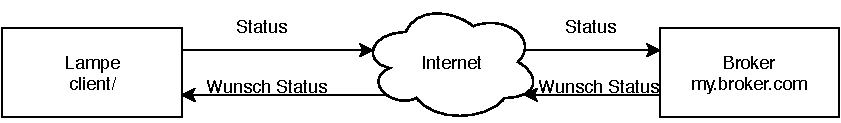
\includepdf[pages=1]{tex/bilder/6_validierung/Szenario.pdf}

\section{Laboraufbau}
    %Warum Virtualisierung/ Virtualisierte Umgebung
    Das Labor wird mithilfe einer Virtualisierungslösung von VMware %
    umgesetzt.  
    %Warum mit ESXI
    
    Die darin enthaltenen System sind die folgenden.
    
    \subsection{Virtualisierung der Geräte}
        \begin{enumerate}
            \item Client: Debian 9, Ressourcen ?, Python 2.X, pip Pakete ?
            \item Broker: Debian 9, Ressourcen ?, Python 3.X, pip Pakete ?
            \item Proxy: 
            Microsoft Windows 10 Pro, Version, 10.0.17763 Build 17763
            \begin{itemize}
                \item Die CPU besteht aus vier virtuellen CPU Kernen.
                \item Es wurde der Maschine 8 GB \ac{RAM} zur Verfügung gestellt.
                \item 50 GB virtuelle Festplatte nach der \ac{VMDK} Format-Spezifikation für \ac{VM}s.
            \end{itemize}
            Frameworks:
            \begin{itemize}
                \item Microsoft Visual C++ 2008
                \item Microsoft Visual C++ 2017
                \item .NET Framework 4.6.1
            \end{itemize}
        \end{enumerate}
    
    \subsection{Netwerk}
    Netzwerk-Setup
    
\section{Ausführung und Bewertung}
Was wird ausgeführt, welche Tests
Als erstes mit einem Client
    Intercepten: werden keine neuen rausgeschickt? werden sie im Web angezeigt?
    Modifizieren: können die im Web modifiziert werden?
    Speichern von Änderungen: können nach der Mod die auch gespeichert werden?
    Neue Nachrichten schicken: können neue geschickt werden?
Als zweites mit zwei Clients

\section{Performance}
    Hier wird die Performance des Proxys analysiert um Hinweise auf Skalierbarkeit und notwendige Ressourcen zu erhalten.
    Folgende Performance-Werte wurden mithilfe des Visual Studio Profilers auf der \ac{VM} Proxy erfasst.
    
    \begin{enumerate}
        \item Ohne Clients:
        Solange das Programm im Leerlauf arbeitet, also nur Events registriert sind die auf die Einwirkung anderer Komponenten warten, benötigt das Programm 19 MB \ac{RAM} und hat eine maximale CPU Auslastung von 1 Prozent.
        \item Mit einem Client:
        Sobald der erste Client sich verbunden hat, wir nur 1 MB mehr \ac{RAM} benötigt, was auf ein Gesamt von 20 MB kommt. Im Gegensatz dazu werden nun nach der ankommenden Nachricht vom \ac{IoT}-Client alle Funktionen des Programms ausgeführt. Dies führt zu einer Erhöhung beim Ausführen der Connect Funktion auf 20 Prozent und anschießend maximal 17 Prozent.
        \item Mit zwei Clients:
        Kommt nun ein weiterer Client dazu, sodass nun zwei Clients mit dem Proxy verbunden sind, steigt der \ac{RAM} Verbrauch weiterhin nur um 1 Prozent auf 21 MB an. Die maximale CPU Auslastung steigt jedoch auf 33 Prozent, was eine Steigerung um 95 Prozent darstellt. Dies ist unter anderem auf ein aktuelles Problem %\cite{https://github.com/Patrick-DE/MQTT-Proxy/issues/3}
        zurückzuführen was dazu führt, dass jeder Client die Antworten aller Clients an den Proxy schickt. Dies bedeutet, dass Antworten des externen Brokers doppelt erfasst und publiziert werden.
        Bei genauerer Analyse beider, am Anstiegen beteiligten Funktionen, ist zu erkennen, dass der größte Ressourcenverbrauch bei den folgenden Funktionen ist.
        \begin{itemize}
            \item Für 30 Prozent der maximalen CPU Auslastung des Programms ist die Connect Funktion verantwortlich. Die Connect Funktion wird aufgerufen, sobald sich ein \ac{IoT}-Client bei dem Proxy registriert. Sie hat mehrere Abhängigkeiten zu weiteren Funktionen die die Methode aufwändiger macht.  
            \item Für 57 Prozent der maximalen CPU Auslastung des Programms ist die Systemfunktion Console.WriteLine() Funktion verantwortlich. Da in diesem Programm viele Informationen an die Konsolenoberfläche zur Information an den Entwickler oder Nutzer weitergereicht werden ist dies die Hauptursache, dass das Programm die oben genannten CPU Auslastung aufweist. Zu bemerken ist jedoch, dass diese nur den maximalen Wert anzeigen, welcher nur vorhanden ist, wenn Nachrichten an den externen Broker weitergeleitet werden.
        \end{itemize}
    \end{enumerate}